\documentclass[tikz,border=10pt]{standalone}
\begin{document}
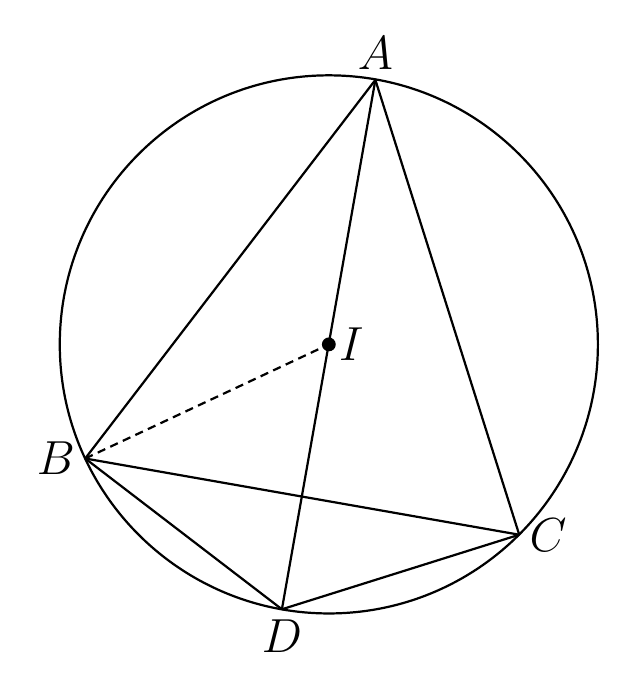
\begin{tikzpicture}[line join=round, line width=0.8pt]
  % Named coordinates (centre I at origin; s = 0.014467 units/px, y flipped)
  \coordinate (I) at (0,0);
  \coordinate (A) at (0.591,3.359);
  \coordinate (B) at (-3.094,-1.449);
  \coordinate (C) at (2.418,-2.417);
  \coordinate (D) at (-0.596,-3.364);

  % Circle, radius 236.17 px -> 3.417 units
  \draw (I) circle[radius=3.417];

  % Solid chords of cyclic quadrilateral ABCD
  \draw (A) -- (B);
  \draw (A) -- (C);
  \draw (A) -- (D);
  \draw (B) -- (C);
  \draw (B) -- (D);
  \draw (C) -- (D);

  % Dashed radius B-I
  \draw[dashed, dash pattern=on 3pt off 2pt] (B) -- (I);

  % Centre point as bold filled dot (~12 px diameter)
  \fill (I) circle (2.5pt);

  % Labels (outside the circle)
  \node[above, font=\fontsize{17}{20.4}\selectfont] at (A) {$A$};
  \node[left, font=\fontsize{17}{20.4}\selectfont] at (B) {$B$};
  \node[right, font=\fontsize{17}{20.4}\selectfont] at (C) {$C$};
  \node[below, font=\fontsize{17}{20.4}\selectfont] at (D) {$D$};
  \node[right, font=\fontsize{17}{20.4}\selectfont] at (I) {$I$};
\end{tikzpicture}
\end{document}